\documentclass[11pt]{article}
\fontfamily{Times}

\usepackage[left=2cm,right=2cm,text={17cm, 24cm},top=2.cm]{geometry}
\usepackage[czech]{babel}
\usepackage[utf8x]{inputenc}
\usepackage{scrextend}
\usepackage{lipsum}
\usepackage{graphicx}
\usepackage{amsthm}
\usepackage{color}


\title{Formální jazyky a překladače \\[0.5 cm] Dokumentace k projektu}		
\author{Marek Kovalčík}								
\date{6. prosince 2017}								

\makeatletter
\let\thetitle\@title
\let\theauthor\@author
\let\thedate\@date
\makeatother

\usepackage{tocloft}

\cftsetindents{section}{0em}{2em}
\cftsetindents{subsection}{0em}{2em}

\renewcommand\cfttoctitlefont{\hfill\Large\bfseries}
\renewcommand\cftaftertoctitle{\hfill\mbox{}}

\setcounter{tocdepth}{2}

\begin{document}
	
	%%%%%%%%%%%%%%%%%%%%%%%%%%%%%%%%%%%%%%%%%%%%%%%%%%%%%%%%%%%%%%%%%%%%%
	
	\begin{titlepage}
		\centering
		\vspace*{0.5 cm}
		
\includegraphics[scale = 0.3]{logo.png}\\[2.0 cm]
		\textsc{\LARGE Vysoké učení technické v Brně}\\[0.3 cm]
		\textsc{\Large Fakulta informačních technologií}\\[2.0 cm]
		\rule{\linewidth}{0.2 mm} \\[2.0 cm]
		{ \huge \bfseries \thetitle}\\[2.0 cm]
		\rule{\linewidth}{0.2 mm} \\[2.0 cm]
		
		\begin{minipage}{0.4\textwidth}
			\begin{flushleft} \large
				\emph{Tým 21, varianta 1}\\[0.5 cm]
				Ondřej Valušek (vedoucí) \\
				David Hříbek	\\
				Dominik Ruta \\
				Marek Kovalčík
			\end{flushleft}
		\end{minipage}
		\begin{minipage}{0.4\textwidth}
			\begin{flushright} \large
				%\emph{Login a ID:} 
				\vspace{1 cm}
				xvalus02, xxxxxx \hspace{1 cm}25\%\\
				xhribe02, xxxxxx \hspace{1 cm}25\%\\
				xrutad00, xxxxxx \hspace{1 cm}25\%\\
				xkoval14, 196248 \hspace{1 cm}25\%\\								
			\end{flushright}
		\end{minipage}\\[2 cm]
		
		{\large \thedate}\\[2 cm]
		
		\vfill
		
	\end{titlepage}
	%%%%%%%%%%%%%%%%%%%%%%%%%%%%%%%%%%%%%%%%%%%%%%%%%%%%%%%%%%%%%%
	\newpage
	\tableofcontents
	\clearpage
	
	
	%%%%%%%%%%%%%%%%%%%%%%%%%%%%%%%%%%%%%%%%%%%%%%%%%%%%%%%%%%%%%%
	
	\section{Organizace a rozdělení práce}
	
	\begin{flushleft}
		Na začátku jsme se domlouvali jaké budeme používat komunikační a vývojové prostředky. Komunikaci jsme prováděli přes sociální síť Facebook a vývoj realizovali pomocí nástroje Git (GitHub).\par
		
		\begin{itemize}
			\item \textbf{Ondřej Valušek} - LL-gramatika, Syntaktická a sémantická analýza
			\item \textbf{David Hříbek} - Lexikální analýza, tabulka symbolů
			\item \textbf{Dominik Ruta} - Syntaktická a sémantická analýza
			\item \textbf{Marek Kovalčík} - Generování cílového kódu, dokumentace
		\end{itemize}	
	\end{flushleft}

	%%%%%%%%%%%%%%%%%%%%%%%%%%%%%%%%%%%%%%%%%%%%%%%%%%%%%%%%%%%%%%
	
	\section{Struktura projektu}
	\subsection{Lexikální analýza}	
	\begin{flushleft}
		Lorem ipsum dolor sit amet, consectetuer adipiscing elit. Maecenas libero. Nullam eget nisl. Maecenas aliquet accumsan leo. Aliquam ante. Cras elementum. Maecenas lorem. In convallis. Donec quis nibh at felis congue commodo. Proin mattis lacinia justo. Nullam rhoncus aliquam metus. Etiam sapien elit, consequat eget, tristique non, venenatis quis, ante. Donec quis nibh at felis congue commodo. Duis ante orci, molestie vitae vehicula venenatis, tincidunt ac pede. Maecenas aliquet accumsan leo.\par	
	\end{flushleft}
	
	\subsection{Syntaktická a sémantická analýza}	
	\begin{flushleft}
		Lorem ipsum dolor sit amet, consectetuer adipiscing elit. Maecenas libero. Nullam eget nisl. Maecenas aliquet accumsan leo. Aliquam ante. Cras elementum. Maecenas lorem. In convallis. Donec quis nibh at felis congue commodo. Proin mattis lacinia justo. Nullam rhoncus aliquam metus. Etiam sapien elit, consequat eget, tristique non, venenatis quis, ante. Donec quis nibh at felis congue commodo. Duis ante orci, molestie vitae vehicula venenatis, tincidunt ac pede. Maecenas aliquet accumsan leo.\par	
	\end{flushleft}
	
	\subsection{Tabulka symbolů}
	\subsubsection{Binární vyhledávací strom}	
	\begin{flushleft}
		Lorem ipsum dolor sit amet, consectetuer adipiscing elit. Maecenas libero. Nullam eget nisl. Maecenas aliquet accumsan leo. Aliquam ante. Cras elementum. Maecenas lorem. In convallis. Donec quis nibh at felis congue commodo. Proin mattis lacinia justo. Nullam rhoncus aliquam metus. Etiam sapien elit, consequat eget, tristique non, venenatis quis, ante. Donec quis nibh at felis congue commodo. Duis ante orci, molestie vitae vehicula venenatis, tincidunt ac pede. Maecenas aliquet accumsan leo.\par	
	\end{flushleft}
	
	\section{Závěr}
	\begin{flushleft}
		Lorem ipsum dolor sit amet, consectetuer adipiscing elit. Maecenas libero. Nullam eget nisl. Maecenas aliquet accumsan leo. Aliquam ante. Cras elementum. Maecenas lorem. In convallis. Donec quis nibh at felis congue commodo. Proin mattis lacinia justo. Nullam rhoncus aliquam metus. Etiam sapien elit, consequat eget, tristique non, venenatis quis, ante. Donec quis nibh at felis congue commodo. Duis ante orci, molestie vitae vehicula venenatis, tincidunt ac pede. Maecenas aliquet accumsan leo.\par
		
		\item \textbf{Počet řádků v projektu:} xxx
		\item \textbf{Počet zdrojových souborů:} xxx
		\item \textbf{Velikost spustitelného souboru:} xxx		
	\end{flushleft}
	
	\vfill
	%%%%%%%%%%%%%%%%%%%%%%%%%%%%%%%%%%%%%%%%%%%%%%%%%%%%%%%%%%%%%%
	\section{Přílohy}
	\subsection{Diagram konečného automatu lexikálního analyzátoru}
	\begin{center}
		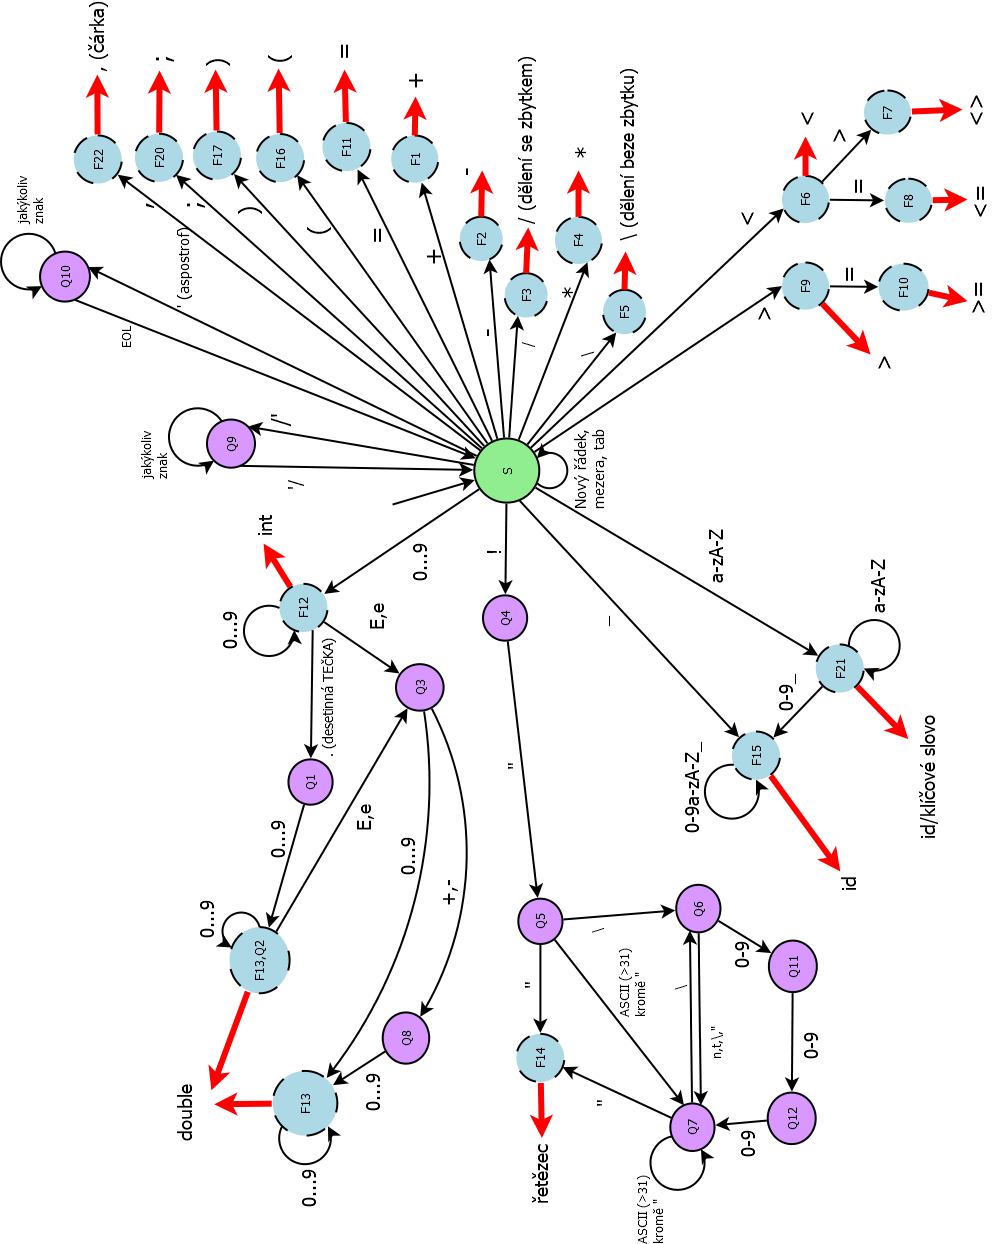
\includegraphics[scale = 0.5]{automat.png}\\
	\end{center}
	\vfill
	%%%%%%%%%%%%%%%%%%%%%%%%%%%%%%%%%%%%%%%%%%%%%%%%%%%%%%%%%%%%%%
	
	\subsection{LL - gramatika}
	\begin{center}
		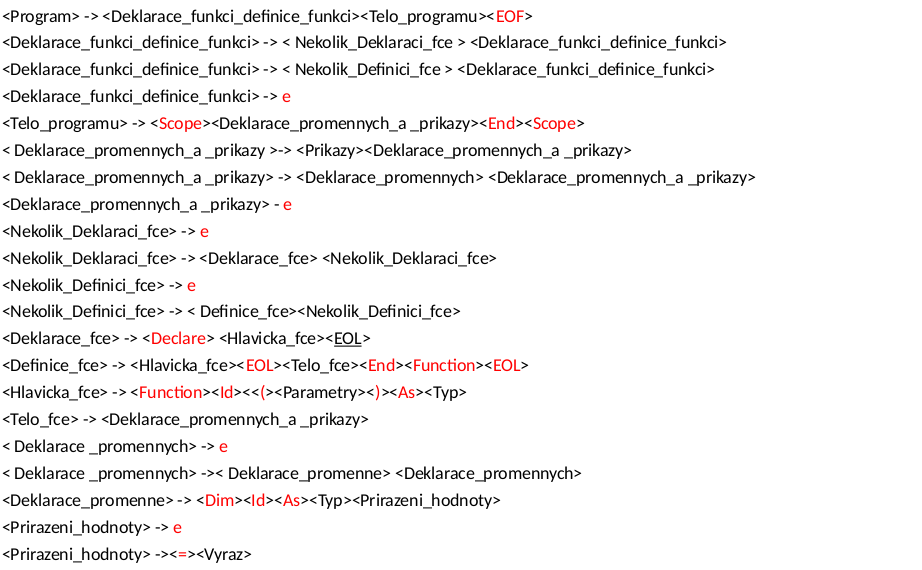
\includegraphics[scale = 0.55]{LL1.png}
		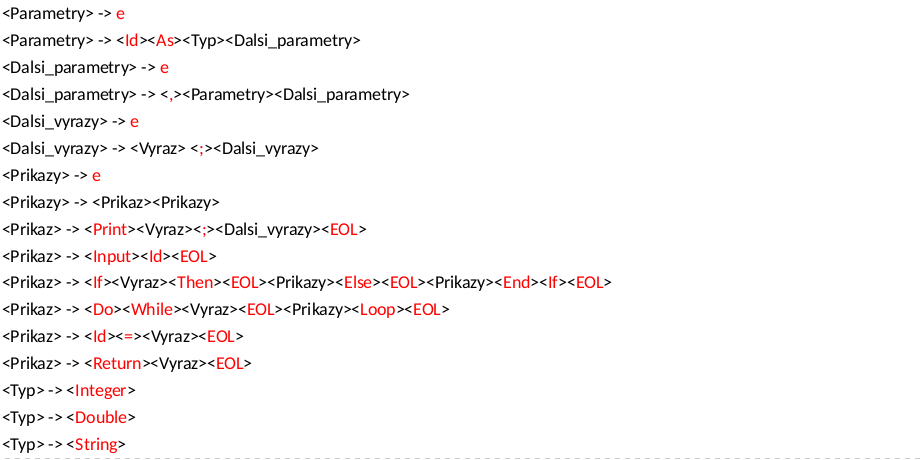
\includegraphics[scale = 0.55]{LL2.png}\\
	\end{center}
	\vfill
	\noindent\hrulefill \\
	\vspace{0.5 cm}
	*\underline{Černě} jsou označeny neterminály a \underline{\textcolor{red}{červeně}} terminály.	
	
	%%%%%%%%%%%%%%%%%%%%%%%%%%%%%%%%%%%%%%%%%%%%%%%%%%%%%%%%%%%%%%
	
	\subsection{LL - tabulka}
	\begin{center}
		%\includegraphics[scale = 0.5]{LL_table.png}\\
	\end{center}
	\vfill
	
	%%%%%%%%%%%%%%%%%%%%%%%%%%%%%%%%%%%%%%%%%%%%%%%%%%%%%%%%%%%%%%
	\newpage
	\subsection{Precedenční tabulka}
	\begin{center}
		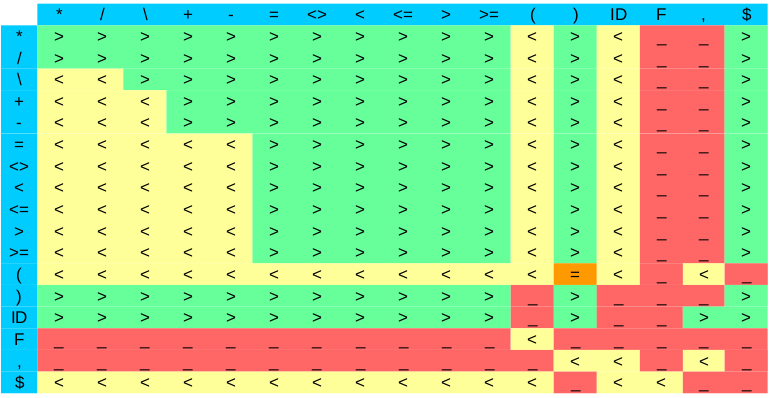
\includegraphics[scale = 0.65]{precendenc_table.png}\\
	\end{center}
	\vfill
	
\end{document}